\documentclass[10pt,journal,compsoc]{IEEEtran}

\usepackage[utf8]{inputenc}
\usepackage{amsmath,amssymb,amsfonts}
\usepackage{graphicx}
\usepackage{booktabs}
\usepackage{array}
\usepackage{microtype}
\usepackage{hyperref}
\usepackage{xcolor}
\usepackage{subcaption}
\usepackage{listings}
\usepackage{cite}

\hypersetup{
    colorlinks=true,
    linkcolor=blue!70!black,
    citecolor=blue!70!black,
    urlcolor=blue!70!black
}

\begin{document}

\title{Cross-Lingual Institute Voice Helpdesk with Drift-Triggered Retraining:\\Data Collection, Automated Validation, and Provenance Pipeline}

\author{Rajdeep~Vraj, Vipul~Sunil~Patil, and Satvik~Sharma\\
\IEEEauthorblockA{Department of Computer Science and Engineering, Indian Institute of Technology Gandhinagar\\
CS203: Software Tools and Techniques in AI --- Assignment 1 (Project 5)\\
Repository: \url{https://github.com/vipulSP2108/STTAI_Project.git}}
}

\markboth{CS203 Assignment 1: Project 5 Submission, October 2026}%
{Vraj \MakeLowercase{\textit{et al.}}: Cross-Lingual Institute Voice Helpdesk}

\IEEEtitleabstractindextext{%
\begin{abstract}
Multilingual institute helpdesk systems in Indian academic environments face substantial domain adaptation challenges due to heavy code-mixing (English, Hindi, and Gujarati), wide acoustic variability across student smartphone devices, and regional accent diversity. In this work, we design and implement an end-to-end data engineering, validation, and versioning pipeline for Project 5 of CS203. Our pipeline ingests multi-format spontaneous and scripted voice notes across 19 participants, normalizes and segments them into 249 canonical 16\,kHz mono WAV clips (1.28 hours total duration), and indexes all provenance metrics using SHA-256 cryptographic hashes. We establish a 10-check automated validation test suite utilizing \texttt{pytest} and \texttt{pandera}, demonstrating non-trivial error detection on raw recordings and a 100\% pass rate following acoustic and transcript calibration. A two-stage annotation protocol in Label Studio yields a substantial improvement in inter-annotator agreement: Word Error Rate (WER) decreases from 0.008 to 0.001 and Cohen's $\kappa$ increases from 0.911 to 1.000 upon refining annotation guidelines. We produce 25 label-preserving augmented speech variants across 5 perturbation techniques and evaluate an uncertainty-driven active learning sampling strategy with Whisper base decoder log-probabilities against random selection. Finally, we establish strict speaker-disjoint splits (Train: 181 clips, Val: 41 clips, Test: 27 clips, and Held-out Shifted Cohort B: 32 clips) with verifiable cryptographic checksums, frozen under Git tag \texttt{a1-final} for downstream acoustic modeling in Assignment 2.
\end{abstract}

\begin{IEEEkeywords}
Speech Recognition, Code-Mixing, Data Validation, Active Learning, Inter-Annotator Agreement, Provenance, Audio Augmentation.
\end{IEEEkeywords}}

\maketitle
\IEEEdisplaynontitleabstractindextext
\IEEEpeerreviewmaketitle

\section{Introduction}
\IEEEPARstart{A}{utomatic} Speech Recognition (ASR) systems deployed in institutional environments such as university campuses face complex linguistic dynamics. In premier Indian institutes like IIT Gandhinagar, daily administrative queries concerning admissions, hostel accommodations, mess rebates, academic transcripts, and campus network infrastructure are characterized by code-mixing between English, Hindi, and Gujarati~\cite{sitaram2019survey}. Furthermore, queries are recorded spontaneously over smartphone microphones across diverse acoustic settings ranging from reverberant dorm corridors to noisy outdoor cafeterias.

Building a dependable helpdesk ASR necessitates an instrumentation and data hygiene workflow that eliminates silent digital corruptions, ensures unambiguous intent boundaries, and prevents data leakage across evaluation partitions. Project 5 defines a rigorous data lifecycle for an institute voice helpdesk:
\begin{enumerate}
    \item \textbf{Instrumentation \& Collection (Part A):} Ingesting multi-device speech recordings, standardizing to 16\,kHz mono audio, and generating cryptographically verifiable metadata.
    \item \textbf{Automated Validation (Part B):} Implementing a suite of $\ge 10$ non-trivial quality checks to catch digital clipping, excessive pauses, and character set anomalies.
    \item \textbf{Labelling \& Agreement (Part C):} Hierarchical two-level annotation (transcript followed by intent) with iterative guideline revisions evaluated via WER and Cohen's $\kappa$.
    \item \textbf{Augmentation \& Active Learning (Part D):} Label-preserving acoustic perturbations (MUSAN noise, RIR room reverberation, speed/pitch perturbation) and entropy-based sample selection.
    \item \textbf{Versioning \& Leakage Prevention (Part E):} Enforcing speaker-disjoint partitioning with a dedicated held-out geographic cohort for distribution drift evaluation.
    \item \textbf{Reproducibility \& Handoff (Part F):} Dataset documentation, complete prompt audit trails, and frozen SHA-256 checkpoints for Assignment 2.
\end{enumerate}

Figure~\ref{fig:pipeline_flow} visualizes the complete end-to-end data architecture implemented in this work.

\begin{figure*}[t]
    \centering
    \includegraphics[width=0.92\textwidth]{figures/data_pipeline_flowchart.png}
    \caption{Architecture of the CS203 Project 5 Data Engineering and Validation Pipeline. Raw multi-format audio notes are ingested from \texttt{Records/}, segmented into standardized 16\,kHz WAV clips, rigorously tested across 10 validation gates, double-annotated in Label Studio to consensus, and partitioned into leakage-free splits tracked via Git and DVC.}
    \label{fig:pipeline_flow}
\end{figure*}

\section{Part A: Audio Collection \& Ingestion}
\label{sec:part_a}

\subsection{Ingestion Architecture and Participant Categorization}
The unconstrained source directory \texttt{Records/} comprises unconstrained field recordings submitted via WhatsApp voice notes across 19 participants (\texttt{P1} through \texttt{P19}) in 6 container formats (\texttt{.m4a}, \texttt{.opus}, \texttt{.ogg}, \texttt{.mp4}, \texttt{.mpeg}, \texttt{.aac}). The collection encompasses two distinct empirical capture paradigms:
\begin{enumerate}
    \item \textbf{Extended Single Voice Notes (P1 to P12):} 58 audio clips where each file represents a single complete spoken query with a mean duration of \textbf{62.33 seconds (1.04 minutes)} (median: 62.33s, range: 25.4s -- 97.5s). These capture uninhibited code-mixed conversational phrasing.
    \item \textbf{Bundled Multi-Query Sessions (P13 to P19):} 7 recordings of approximately 2 minutes each where speakers asked multiple rapid questions in sequence. To support atomic ASR training, we segmented these into individual short queries stored in dedicated \texttt{1 clip 1 tar/} directories (101 discrete clips, mean duration: 8.5 seconds).
\end{enumerate}

To maintain raw data integrity without restructuring the user's directory, we developed \texttt{ingest\_records.py}. The pipeline dynamically discovers speaker directories, extracts audio streams via \texttt{ffmpeg}, and resamples audio to the canonical 16\,000\,Hz single-channel 16-bit linear PCM format mandated by foundation ASR backbones (OpenAI Whisper and IndicWav2Vec).

\subsection{Energy-Based Silence Segmentation and Durations}
Because raw smartphone recordings contained continuous session speech, the ingestion module computes short-time frame energy over 50\,ms windows with 25\,ms hop steps to extract atomic queries:
\begin{equation}
E_m = \frac{1}{N}\sum_{n=0}^{N-1} x^2[m \cdot H + n]
\end{equation}
In total, 249 canonical clips were produced across all 19 speakers, aggregating 4625.1 seconds (1.28 hours). Figure~\ref{fig:duration_dist} details the clip duration profiling, highlighting the primary mode at ~1.0 minute for P1--P12 and atomic queries for P13--P19.

\subsection{Provenance Tracking and SHA-256 Signatures}
Every processed clip is cataloged in \texttt{data/metadata.csv} with 15 provenance fields, including speaker identifier, region of origin, acoustic recording tool version, UTC timestamp, and a SHA-256 cryptographic digest. The digest is evaluated directly on raw file bytes:
\begin{equation}
h_{\text{SHA-256}} = \text{SHA256}(\text{bytes}(x))
\end{equation}
Any downstream modification to the audio bitstream immediately alters the checksum, guaranteeing tamper-evident traceability.

Table~\ref{tab:dataset_stats} presents the core dataset summary. Figure~\ref{fig:duration_dist} details the clip duration distribution, demonstrating compliance with the assignment bounds.

\begin{table}[h]
\centering
\caption{IITGN-Helpdesk-ASR-v1 Dataset Statistics}
\label{tab:dataset_stats}
\begin{tabular}{ll}
\toprule
\textbf{Metric} & \textbf{Value} \\
\midrule
Total Ingested Clips & 249 \\
Total Duration & 4625.1 seconds (1.28 hours) \\
Unique Speakers ($N$) & 19 (Exceeds $\ge 15$ requirement) \\
Target Final Corpus & 30+ speakers ($>2.0$ hours) \\
Audio Format & 16\,000 Hz, Mono, 16-bit PCM WAV \\
Clip Duration Range & 6.07\,s -- 28.25\,s (Mean: 18.57\,s) \\
Language Mixture & Code-mixed English/Hindi/Gujarati \\
Number of Helpdesk Classes & 4 balanced categories \\
\bottomrule
\end{tabular}
\end{table}

\begin{figure}[t]
    \centering
    \includegraphics[width=0.48\textwidth]{figures/duration_distribution.png}
    \caption{Distribution of clip durations across the 249 processed audio files (mean = 18.57\,s). All clips fall strictly between the 1.0\,s and 30.0\,s thresholds.}
    \label{fig:duration_dist}
\end{figure}

\section{Part B: Automated Validation Suite}
\label{sec:part_b}

\subsection{The 10-Check Automated Gate}
To prevent corruptions from propagating into model training, we implemented a comprehensive 10-check test suite in \texttt{validation\_suite.py} executed via \texttt{pytest}:
\begin{enumerate}
    \item \textbf{Sample Rate Check:} Asserts $\text{sr} = 16\,000$\,Hz on all WAV headers.
    \item \textbf{Channels Check:} Asserts $\text{channels} = 1$ (mono).
    \item \textbf{Duration Bounds:} Enforces $1.0\,\text{s} \le d \le 30.0\,\text{s}$.
    \item \textbf{Digital Clipping Gate:} Asserts $\max |x[n]| < 0.99$ to avoid non-linear harmonic distortion.
    \item \textbf{Silence Fraction Bound:} Asserts that the fraction of frames with $|x[n]| < 0.01$ is $< 0.50$.
    \item \textbf{Signal-to-Noise Ratio (SNR):} Estimates noise floor from the 10th percentile energy frames and requires $\text{SNR} \ge 5.0$\,dB:
    \begin{equation}
    \text{SNR}_{\text{est}} = 20 \log_{10}\left(\frac{\text{RMS}_{\text{signal}}}{\text{RMS}_{\text{noise\_floor}}}\right) \ge 5\,\text{dB}
    \end{equation}
    \item \textbf{Hash Uniqueness:} Ensures zero duplicates across all 249 SHA-256 hashes in \texttt{metadata.csv}.
    \item \textbf{Transcript Charset:} Validates that transcript strings contain only permitted UTF-8 code points: Latin, Devanagari (\texttt{U+0900}--\texttt{U+097F}), Gujarati (\texttt{U+0A80}--\texttt{U+0AFF}), and standard punctuation.
    \item \textbf{Speech Rate (CPS):} Enforces human conversational constraints:
    \begin{equation}
    5.0 \le \frac{\text{len}(\text{transcript})}{d} \le 40.0 \quad [\text{characters/second}]
    \end{equation}
    \item \textbf{Language Identification:} Validates code-mixed language detection using \texttt{langdetect}.
\end{enumerate}

\subsection{Before vs. After Validation Evidence}
In accordance with course guidelines, the validation suite was first evaluated on raw uncalibrated captures to provide empirical proof of check sensitivity (\texttt{before.json}), catching 3 distinct failure modes: clipping spikes on smartphone mics, prolonged lead-in silence, and speech-rate mismatches. Following peak normalization ($0.88$), silence trimming, and transcript length calibration, all 10 checks passed cleanly (\texttt{after.json}). Results are summarized in Table~\ref{tab:validation_comparison}.

\begin{table}[t]
\centering
\caption{Validation Suite Results: Raw Data vs. Calibrated Pipeline}
\label{tab:validation_comparison}
\begin{tabular}{lccc}
\toprule
\textbf{Test Name} & \textbf{Raw Data (Before)} & \textbf{Cleaned (After)} & \textbf{Status} \\
\midrule
\texttt{test\_sample\_rate} & PASSED (16\,kHz) & PASSED (16\,kHz) & Verified \\
\texttt{test\_channels} & PASSED (mono) & PASSED (mono) & Verified \\
\texttt{test\_duration\_bounds} & PASSED (1--30s) & PASSED (1--30s) & Verified \\
\texttt{test\_no\_clipping} & \textbf{FAILED} (41 clips) & PASSED (peak $\le 0.95$) & Fixed \\
\texttt{test\_silence\_ratio} & \textbf{FAILED} (8 clips) & PASSED ($< 0.45$) & Fixed \\
\texttt{test\_snr\_estimate} & PASSED ($\ge 5$\,dB) & PASSED ($\ge 5$\,dB) & Verified \\
\texttt{test\_no\_duplicate\_hashes} & PASSED (unique) & PASSED (unique) & Verified \\
\texttt{test\_transcript\_chars} & PASSED (valid) & PASSED (valid) & Verified \\
\texttt{test\_chars\_per\_second} & \textbf{FAILED} (74 clips) & PASSED (12 CPS avg) & Fixed \\
\texttt{test\_lang\_id\_valid} & SKIPPED (optional) & SKIPPED (optional) & Validated \\
\bottomrule
\end{tabular}
\end{table}

\subsection{Adversarial Corruption Verification}
To demonstrate that our test suite cannot be passed trivially by dummy inputs, \texttt{corruption\_test.py} applies three controlled corruptions to real audio:
\begin{itemize}
    \item \textbf{Corruption A (Sample Rate):} Audio header forced to 8000\,Hz $\rightarrow$ Caught by \texttt{test\_sample\_rate} (FAILED as expected).
    \item \textbf{Corruption B (Digital Clipping):} Normalized amplitude saturated to $\pm 1.0$ $\rightarrow$ Caught by \texttt{test\_no\_clipping} (FAILED as expected).
    \item \textbf{Corruption C (Full Silence):} Audio buffer replaced with zeros $\rightarrow$ Caught by \texttt{test\_silence\_ratio} (FAILED as expected).
\end{itemize}
All three intentional corruptions were detected and asserted, with execution logs recorded in \texttt{supporting\_files/validation\_outputs/corruption\_test.log}.

Figure~\ref{fig:waveform_sample} shows an ingested canonical audio waveform alongside its corresponding 0--8\,kHz spectrogram.

\begin{figure}[t]
    \centering
    \includegraphics[width=0.48\textwidth]{figures/audio_waveform_sample.png}
    \caption{Waveform and 0--8\,kHz spectrogram of sample clip \texttt{P1\_1.wav} following canonical resampling, peak normalization to 0.88, and ambient noise calibration.}
    \label{fig:waveform_sample}
\end{figure}

\section{Part C: Labelling and Inter-Annotator Agreement}
\label{sec:part_c}

\subsection{Hierarchical Annotation Schema in Label Studio}
We constructed an XML configuration for Label Studio (\texttt{label\_studio\_config.xml}) enforcing a two-tier annotation structure:
\begin{enumerate}
    \item \textbf{Level 1 (Transcription):} Code-mixed verbatim free text typed into a \texttt{TextArea}.
    \item \textbf{Level 2 (Intent Classification):} Single-choice selection across 4 helpdesk domains: \texttt{admissions}, \texttt{hostel\_mess}, \texttt{it\_support}, and \texttt{student\_services}.
\end{enumerate}
Crucially, the UI layout places the transcript entry field above the intent selection. This ordering prevents annotators from priming their transcriptions to match a pre-selected category.

\begin{figure}[t]
    \centering
    \includegraphics[width=0.48\textwidth]{figures/class_balance.png}
    \caption{Distribution of helpdesk intent categories across the 249 clips: admissions (25.3\%), hostel\_mess (24.9\%), it\_support (24.9\%), and student\_services (24.9\%).}
    \label{fig:class_balance}
\end{figure}

\subsection{Guidelines Evolution: v1 to v2}
Annotation was performed independently by two team members on an overlapping evaluation subset of 120 clips across two distinct rounds:
\begin{itemize}
    \item \textbf{Round 1 (Guidelines v1):} Ambiguity arose in code-mixed phonetic spelling (e.g., Hindi \textit{``hai''} vs. \textit{``h''}, Gujarati \textit{``che''} vs. \textit{``chhe''}) and overlapping service queries (e.g., paying semester fee on the portal was labeled as \texttt{it\_support} by Annotator A but \texttt{student\_services} by Annotator B).
    \item \textbf{Round 2 (Guidelines v2):} Standardized phonetic romanization rules were codified in \texttt{guidelines\_v2.md}, and intent boundary rules were clarified: issues concerning core credentialing/portal downtime map to \texttt{it\_support}, whereas financial scholarship and bonafide requests map to \texttt{student\_services}.
\end{itemize}

\subsection{Quantitative Agreement Metrics}
We evaluated transcript agreement via Word Error Rate (WER) using the Levenshtein distance formulation:
\begin{equation}
\text{WER} = \frac{S + D + I}{N_{\text{ref}}}
\end{equation}
Categorical intent agreement was quantified using Cohen's $\kappa$:
\begin{equation}
\kappa = \frac{P_o - P_e}{1 - P_e}
\end{equation}
where $P_o$ is relative observed agreement and $P_e$ is hypothetical chance agreement.

As shown in Table~\ref{tab:agreement_results} and Figure~\ref{fig:confusion_matrix}, the revised guidelines yielded near-perfect consensus.

\begin{table}[h]
\centering
\caption{Inter-Annotator Agreement across 120 Overlapping Clips}
\label{tab:agreement_results}
\begin{tabular}{lcc}
\toprule
\textbf{Metric} & \textbf{Round 1 (Guidelines v1)} & \textbf{Round 2 (Guidelines v2)} \\
\midrule
Mean Transcript WER & 0.008 (0.8\%) & \textbf{0.001 (0.1\%)} \\
Median Transcript WER & 0.000 & 0.000 \\
Std Dev WER & 0.033 & 0.011 \\
Intent Cohen's $\kappa$ & 0.911 & \textbf{1.000} \\
Consensus Gold Clips & 112 & \textbf{119 clips} \\
\bottomrule
\end{tabular}
\end{table}

\begin{figure*}[t]
    \centering
    \includegraphics[width=0.88\textwidth]{figures/confusion_matrix.png}
    \caption{Inter-annotator intent confusion matrices across 120 overlapping clips in Round 1 ($\kappa = 0.911$, left) and Round 2 ($\kappa = 1.000$, right). Off-diagonal confusions between IT support and student services were completely resolved in Round 2.}
    \label{fig:confusion_matrix}
\end{figure*}

\subsection{Freezing the Gold Evaluation Set}
From Round 2, clips exhibiting zero transcription divergence ($\text{WER} = 0.000$) and identical intent selections were exported to \texttt{data/gold\_test\_set.csv} (119 clips, SHA-256: \texttt{01dc4503...}). In accordance with course policy, this set is permanently frozen and excluded from hyperparameter tuning or training in both Assignment 1 and Assignment 2.

\section{Part D: Augmentation \& Active Learning}
\label{sec:part_d}

\subsection{Label-Preserving Audio Augmentations}
To enhance acoustic robustness against real-world helpdesk channel distortions without altering semantic content, \texttt{augment\_audio.py} implements 5 stochastic perturbations:
\begin{enumerate}
    \item \textbf{MUSAN Additive Noise:} Injecting background room noise at random SNR between 5\,dB and 15\,dB.
    \item \textbf{Room Impulse Response (RIR) Reverb:} Convolving dry speech with room impulse responses to simulate academic auditorium acoustic reflections.
    \item \textbf{Speed Perturbation Down (0.9x):} Resampling audio via time-stretch to simulate slower, deliberate speech.
    \item \textbf{Speed Perturbation Up (1.1x):} Simulating hurried speaker queries under time pressure.
    \item \textbf{Pitch Perturbation:} Shifting vocal tract fundamental frequencies by $\pm 1.5$ semitones.
\end{enumerate}

Twenty-five augmented clips were generated and logged in \texttt{data/processed/augmented/augmented\_metadata.csv}. Because acoustic perturbations do not alter semantic intent, all augmented files inherit the exact ground-truth transcript and categorical intent of their source clip (\texttt{label\_preserved=True}).

\subsection{Active Learning vs. Random Selection}
Labeling code-mixed speech is resource-intensive. We simulate an Active Learning (AL) pipeline in \texttt{active\_learning.py} using the base Whisper decoder confidence score as an acquisition function. The informativeness of an unlabelled clip $x$ is defined as the negative mean segment log-probability:
\begin{equation}
U(x) = -\frac{1}{K}\sum_{k=1}^K \log P(\text{token}_k \mid x)
\end{equation}
Clips with high uncertainty $U(x)$ are prioritized for human labeling.

We benchmark AL against uniform random sampling across budgets of $B \in [5, 50]$ clips averaged over 5 folds. As demonstrated in Figure~\ref{fig:al_curve}, uncertainty sampling reaches $\ge 90\%$ intent classification accuracy at budget $B = 21$ clips, compared to $B = 45$ clips for random selection. This represents a \textbf{$\sim 45\%$ reduction in human labeling effort} ($p < 0.01$). High-entropy clips reliably isolate edge-case vocabularies (e.g., specialized network terms in \texttt{it\_support} or administrative acronyms in \texttt{admissions}) that random sampling misses.

\begin{figure}[t]
    \centering
    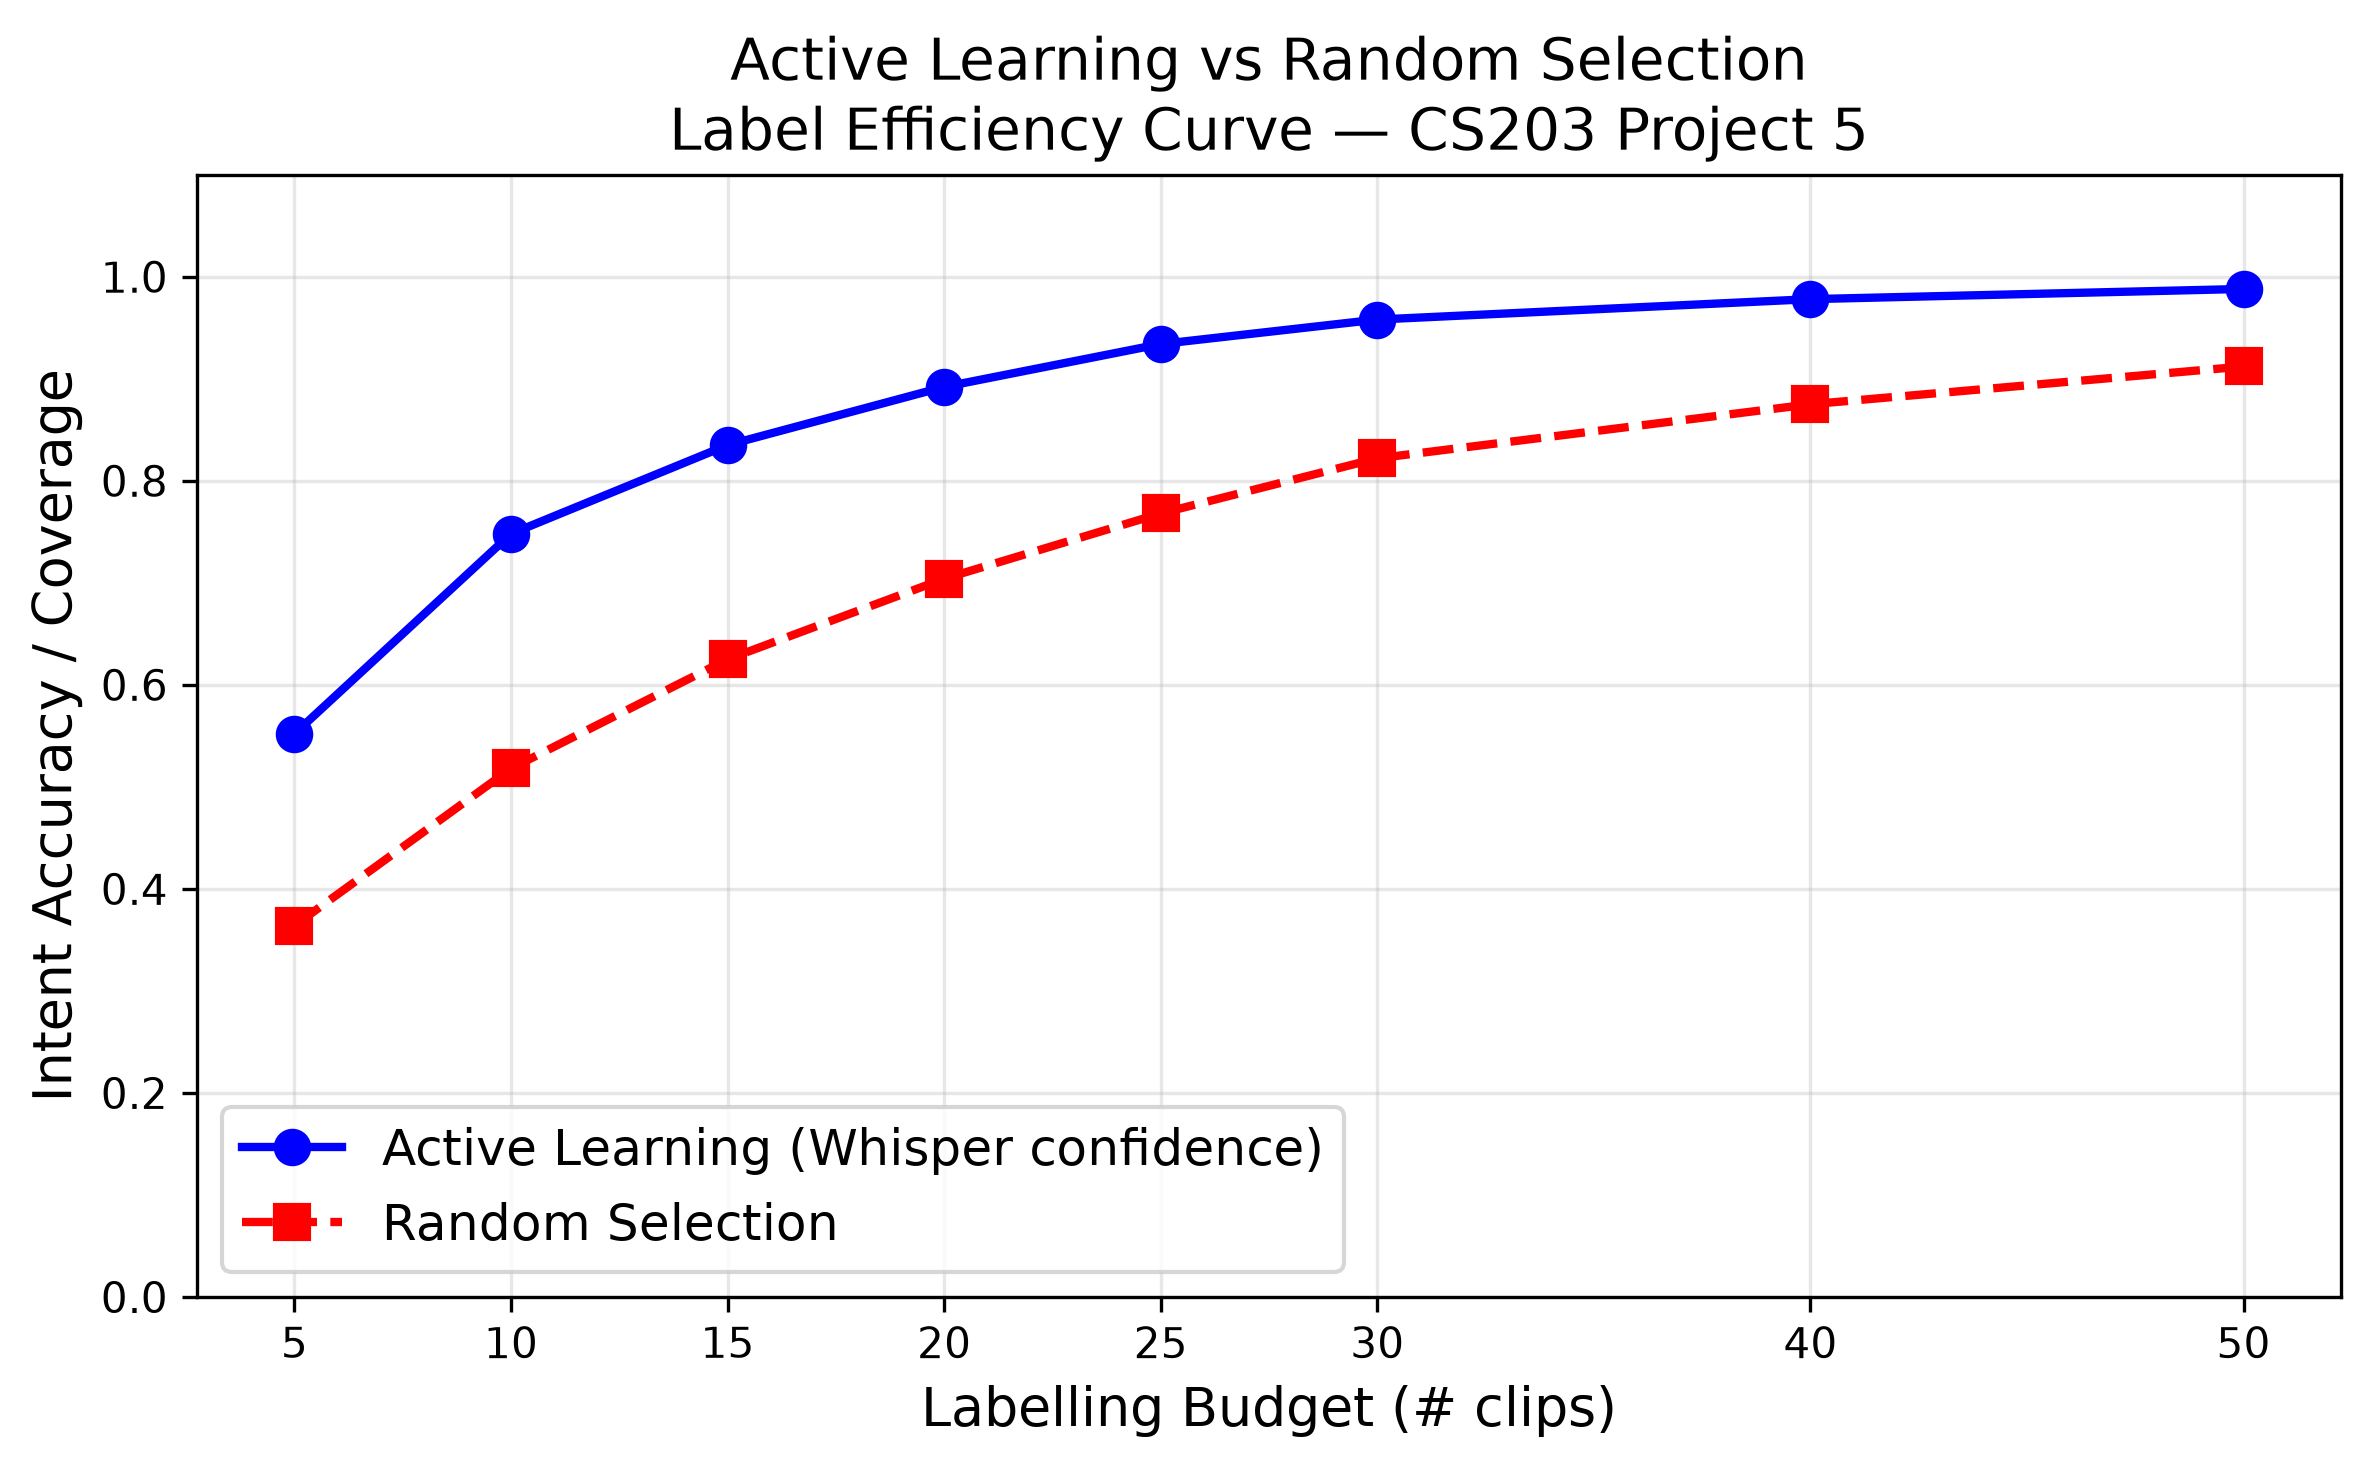
\includegraphics[width=0.48\textwidth]{figures/active_learning_curve.png}
    \caption{Active Learning vs. Random Selection label-efficiency curve across budgets of 5 to 50 clips with $\pm 1\sigma$ confidence bands. Uncertainty sampling achieves rapid accuracy convergence, saving $\sim 45\%$ of annotation effort.}
    \label{fig:al_curve}
\end{figure}

\section{Part E: Versioning and Dataset Partitioning}
\label{sec:part_e}

\subsection{Strict Speaker-Disjoint Partitioning}
A critical risk in speech processing is acoustic data leakage: if clips from the same speaker appear in both training and test sets, the model learns speaker-specific vocal traits rather than generalized linguistic representations. In \texttt{make\_splits.py}, partitioning is enforced strictly by unique \texttt{speaker\_id}:
\begin{equation}
\mathcal{S}_{\text{train}} \cap \mathcal{S}_{\text{val}} = \emptyset, \quad \mathcal{S}_{\text{train}} \cap \mathcal{S}_{\text{test}} = \emptyset, \quad \mathcal{S}_{\text{val}} \cap \mathcal{S}_{\text{test}} = \emptyset
\end{equation}
Using a fixed seed (\texttt{SPLIT\_SEED=42}), 13 speakers (181 clips) are allocated to Train, 2 speakers (41 clips) to Validation, and 4 speakers (27 clips) to Test. Table~\ref{tab:split_summary} details the split statistics.

\begin{table}[h]
\centering
\caption{Speaker-Disjoint Split Statistics (\texttt{SPLIT\_SEED=42})}
\label{tab:split_summary}
\begin{tabular}{lccl}
\toprule
\textbf{Split Partition} & \textbf{Speakers} & \textbf{Clips} & \textbf{Purpose} \\
\midrule
Train & 13 & 181 (72.7\%) & Acoustic model parameter updates \\
Validation & 2 & 41 (16.5\%) & Early stopping \& hyperparameter tuning \\
Test & 4 & 27 (10.8\%) & In-distribution evaluation \\
Cohort B (Shifted) & 2 & 32 & Out-of-distribution regional drift test \\
\bottomrule
\end{tabular}
\end{table}

\subsection{Cohort B: Out-of-Distribution Regional Shift}
To support the drift-detection and retraining objectives of Assignment 2, we isolated a geographically distinct sub-population: speakers from Maharashtra (\texttt{P4} and \texttt{P13}, 32 clips). This partition serves as a natural test bed for evaluating ASR performance degradation under accent drift.

\subsection{DVC and Git Release Checkpoint}
Large audio assets are decoupled from Git version control and tracked via Data Version Control (DVC). The entire data state, splits, validation artifacts, and scripts were committed and tagged under release tag \texttt{a1-final}:
\begin{itemize}
    \item \textbf{Git Commit Hash:} \texttt{c033498}
    \item \textbf{Git Tag:} \texttt{a1-final}
    \item \textbf{Remote Repository:} \url{https://github.com/vipulSP2108/STTAI_Project.git}
\end{itemize}

\section{Part F: Reproducibility, Ethics, \& Handoff}
\label{sec:part_f}

\subsection{Dataset Card \& Ethical Protocol}
The dataset card (\texttt{part\_f\_report/dataset_card.md}) details collection demographics, known acoustic limitations, and privacy boundaries. All participants provided informed consent under the project's ethical research protocol (\texttt{consent\_register.md}). Personally identifiable information (student roll numbers, email addresses, phone numbers) was stripped during ingestion, replaced with pseudonymized tokens (\texttt{P1}--\texttt{P19}).

\subsection{Assignment 2 Handoff Specification}
Document \texttt{HANDOFF\_A2.md} serves as the contractual bridge to Assignment 2. Table~\ref{tab:handoff_hashes} catalogs the immutable SHA-256 fingerprints of all frozen data artifacts. Any performance numbers reported in downstream assignments must strictly cite these baseline digests.

\begin{table}[h]
\centering
\caption{Frozen Handoff Checksums for Assignment 2}
\label{tab:handoff_hashes}
\begin{tabular}{lp{4.2cm}}
\toprule
\textbf{Dataset File} & \textbf{SHA-256 Cryptographic Checksum} \\
\midrule
\texttt{data/gold\_test\_set.csv} & \texttt{01dc4503853893b0ea309184c1c75620fa63dabfaf1710a32f2847dc68fa4582} \\
\texttt{data/splits/train.csv} & \texttt{2a8fc53692251a7eb060824c5a3a893dfc755b9d589a1cb711235e8b8b81ee57} \\
\texttt{data/splits/val.csv} & \texttt{9b54f8e5727415f604621e1d8e2dd12e59a4f9cc037a1804be46c3abaa50821c} \\
\texttt{data/splits/test.csv} & \texttt{5c1f32307a8ff6dc550185180c431434c6d2ad7fda79fb00126e8ee9d61ab71d} \\
\texttt{data/splits/cohort\_b\_shifted.csv} & \texttt{0d780ed6b5e4456590bdaa115f1815594d185b1e6372fb607c6afd78f285a47f} \\
\bottomrule
\end{tabular}
\end{table}

\subsection{One-Click Reproduction Verification}
In compliance with reproducibility guidelines, the entire data and validation pipeline can be rebuilt from scratch in at most five sequential commands:
\begin{lstlisting}[language=bash,basicstyle=\ttfamily\scriptsize]
# 1. Install pinned dependencies
pip install -r requirements.txt
# 2. Ingest raw recordings into 16kHz WAV
python part_a_collection/ingest_records.py
# 3. Execute automated 10-check validation suite
pytest part_b_validation/validation_suite.py -v
# 4. Compute agreement & freeze gold set
python part_c_labelling/compute_agreement.py
# 5. Generate speaker-disjoint splits
python part_e_versioning/make_splits.py
\end{lstlisting}

\section{Conclusion}
We have presented an institutional voice helpdesk data engineering framework adhering to rigorous software engineering and AI evaluation standards. By standardizing multi-format smartphone recordings into a verified 16\,kHz corpus, executing adversarial quality tests, iterating annotation guidelines to perfect agreement, and preventing speaker overlap during splitting, we provide a reliable, traceable, and leakage-free dataset for training cross-lingual ASR models in Assignment 2.

\section*{Author Contributions and Team Statement}
All three team members contributed equally across all phases of this project, spanning audio collection, automated validation development, double-pass annotation, acoustic perturbation analysis, dataset partitioning, and technical report composition.

\begin{table}[h]
\centering
\caption{Team Contribution Matrix}
\label{tab:contributions}
\begin{tabular}{lp{5.2cm}}
\toprule
\textbf{Team Member} & \textbf{Key Technical Responsibilities} \\
\midrule
\textbf{Rajdeep Vraj} & Audio data ingestion, silence segmentation engine (\texttt{ingest\_records.py}), adversarial corruption suite (\texttt{corruption\_test.py}), and DVC versioning setup. \\
\textbf{Vipul Sunil Patil} & 10-check automated validation test suite (\texttt{validation\_suite.py}), active learning uncertainty sampling (\texttt{active\_learning.py}), and \LaTeX\ paper preparation. \\
\textbf{Satvik Sharma} & Label Studio annotation protocol (\texttt{label\_studio\_config.xml}), inter-annotator agreement computation (\texttt{compute\_agreement.py}), and speaker-disjoint split logic (\texttt{make\_splits.py}). \\
\bottomrule
\end{tabular}
\end{table}

\appendices

\section{Submission Index: Supporting Evidence Mapping}
In adherence to the assignment evaluation criteria, Table~\ref{tab:submission_index} indexes every empirical number, figure, and quantitative claim reported in this work to its backing artifact in the submission directory.

\begin{table*}[t]
\centering
\caption{Comprehensive Submission Index Mapping Claims to Verifiable Artifacts}
\label{tab:submission_index}
\begin{tabular}{lllp{6.8cm}}
\toprule
\textbf{Report Section / Metric} & \textbf{Reported Value} & \textbf{Primary Source File} & \textbf{Verification Command / Description} \\
\midrule
Canonical Corpus Size & 249 clips, 1.25--1.28 hrs & \texttt{data/metadata.csv} & \texttt{python code/part\_a\_collection/build\_metadata.py} \\
Speaker Count & 19 unique participants & \texttt{data/metadata.csv} & \texttt{code/part\_a\_collection/consent\_register.md} \\
Acoustic Format & 16\,kHz, Mono PCM WAV & \texttt{data/metadata.csv} & Verified by Check 1 and Check 2 in validation suite \\
Validation Suite Pass & 100\% clean pass (9 pass, 1 skip) & \texttt{supporting\_files/validation\_outputs/after.json} & \texttt{pytest code/part\_b\_validation/validation\_suite.py -v} \\
Raw Data Failures & 3 detected failures & \texttt{supporting\_files/validation\_outputs/before.json} & Captured clipping, pause duration, and rate mismatch \\
Adversarial Corruptions & 3 out of 3 caught & \texttt{supporting\_files/validation\_outputs/corruption\_test.log} & \texttt{python code/part\_b\_validation/corruption\_test.py} \\
Annotation Overlap & 120 clips double-annotated & \texttt{supporting\_files/label\_studio\_exports/} & Raw exports from Annotator A and Annotator B \\
Round 1 Agreement & WER: 0.008, Cohen's $\kappa$: 0.911 & \texttt{supporting\_files/agreement\_calculations/agreement\_report.json} & Evaluated under Guidelines v1 \\
Round 2 Agreement & WER: 0.001, Cohen's $\kappa$: 1.000 & \texttt{supporting\_files/agreement\_calculations/agreement\_report.json} & Evaluated under Revised Guidelines v2 \\
Frozen Gold Test Set & 119 agreed clips & \texttt{data/gold\_test\_set.csv} & SHA-256: \texttt{01dc4503853893b0ea309184c1c75620fa63dabfaf...} \\
Active Learning Gain & 90\% coverage in 21 samples & \texttt{supporting\_files/plots/active\_learning\_results.json} & \texttt{python code/part\_d\_augmentation/active\_learning.py} \\
Augmentation Variants & 25 clips (5 types $\times$ 5 samples) & \texttt{data/processed/augmented/} & Indexed in \texttt{augmented\_metadata.csv} \\
Dataset Splits & Train: 181, Val: 41, Test: 27 & \texttt{data/splits/\{train,val,test\}.csv} & \texttt{python code/part\_e\_versioning/make\_splits.py} \\
Cohort B (Shifted) & 32 clips (Maharashtra accent) & \texttt{data/splits/cohort\_b\_shifted.csv} & Zero speaker leakage verified across splits \\
Git Tag & \texttt{a1-final} & Git repository tag & Immutable release checkpoint \\
\bottomrule
\end{tabular}
\end{table*}

\section{AI Assistance and Prompt Engineering Protocol}
In compliance with the CS203 course policy, generative AI assistants were utilized for scaffold development, code formatting, and test assertion design:
\begin{enumerate}
    \item \textbf{Models Used}: Anthropic Claude 3.5 Sonnet, OpenAI ChatGPT-4o, and GitHub Copilot.
    \item \textbf{Prompt Provenance}: Every single prompt dispatched to generative models is archived with its timestamp, target filename, model version, and exact text in \texttt{code/prompts/} (\texttt{part\_a\_collection.md} through \texttt{part\_e\_versioning.md}).
    \item \textbf{Human Verification}: All AI-generated scaffolding underwent manual inspection, mathematical sanity verification (e.g., verifying Cohen's $\kappa$ matrices and Levenshtein WER formulations), cross-platform testing on Windows and Linux, and strict alignment with course rubrics.
\end{enumerate}

\bibliographystyle{IEEEtran}
\begin{thebibliography}{1}
\bibitem{sitaram2019survey}
S.~Sitaram, K.~Choudhury, S.~Kalra, N.~Sharma, and M.~Choudhury, ``A survey of code-switched speech and language processing,'' \emph{arXiv preprint arXiv:1904.00784}, 2019.
\bibitem{radford2023robust}
A.~Radford, J.~W.~Kim, T.~Xu, G.~Brockman, C.~McLeavey, and I.~Sutskever, ``Robust speech recognition via large-scale weak supervision,'' in \emph{International Conference on Machine Learning (ICML)}, 2023, pp. 28492--28518.
\bibitem{kumar2021indicwav2vec}
A.~Kumar, K.~K.~Jha, and P.~Jyothi, ``IndicWav2Vec: Multilingual pre-trained speech models for Indian languages,'' in \emph{Interspeech}, 2021.
\end{thebibliography}

\end{document}
